\PassOptionsToPackage{unicode=true}{hyperref} % options for packages loaded elsewhere
\PassOptionsToPackage{hyphens}{url}
%
\documentclass[english,doc]{apa6}
\usepackage{lmodern}
\usepackage{amssymb,amsmath}
\usepackage{ifxetex,ifluatex}
\usepackage{fixltx2e} % provides \textsubscript
\ifnum 0\ifxetex 1\fi\ifluatex 1\fi=0 % if pdftex
  \usepackage[T1]{fontenc}
  \usepackage[utf8]{inputenc}
  \usepackage{textcomp} % provides euro and other symbols
\else % if luatex or xelatex
  \usepackage{unicode-math}
  \defaultfontfeatures{Ligatures=TeX,Scale=MatchLowercase}
\fi
% use upquote if available, for straight quotes in verbatim environments
\IfFileExists{upquote.sty}{\usepackage{upquote}}{}
% use microtype if available
\IfFileExists{microtype.sty}{%
\usepackage[]{microtype}
\UseMicrotypeSet[protrusion]{basicmath} % disable protrusion for tt fonts
}{}
\IfFileExists{parskip.sty}{%
\usepackage{parskip}
}{% else
\setlength{\parindent}{0pt}
\setlength{\parskip}{6pt plus 2pt minus 1pt}
}
\usepackage{hyperref}
\hypersetup{
            pdftitle={If mathematical psychology did not exist we would need to invent it: A case study in cumulative theoretical development in psychology},
            pdfkeywords={psychological theory, inductive generalization, mathematical psychology, cognitive modelling},
            pdfborder={0 0 0},
            breaklinks=true}
\urlstyle{same}  % don't use monospace font for urls
\usepackage{graphicx,grffile}
\makeatletter
\def\maxwidth{\ifdim\Gin@nat@width>\linewidth\linewidth\else\Gin@nat@width\fi}
\def\maxheight{\ifdim\Gin@nat@height>\textheight\textheight\else\Gin@nat@height\fi}
\makeatother
% Scale images if necessary, so that they will not overflow the page
% margins by default, and it is still possible to overwrite the defaults
% using explicit options in \includegraphics[width, height, ...]{}
\setkeys{Gin}{width=\maxwidth,height=\maxheight,keepaspectratio}
\setlength{\emergencystretch}{3em}  % prevent overfull lines
\providecommand{\tightlist}{%
  \setlength{\itemsep}{0pt}\setlength{\parskip}{0pt}}
\setcounter{secnumdepth}{0}

% set default figure placement to htbp
\makeatletter
\def\fps@figure{htbp}
\makeatother

% Manuscript styling
\usepackage{upgreek}
\captionsetup{font=singlespacing,justification=justified}

% Table formatting
\usepackage{longtable}
\usepackage{lscape}
% \usepackage[counterclockwise]{rotating}   % Landscape page setup for large tables
\usepackage{multirow}		% Table styling
\usepackage{tabularx}		% Control Column width
\usepackage[flushleft]{threeparttable}	% Allows for three part tables with a specified notes section
\usepackage{threeparttablex}            % Lets threeparttable work with longtable

% Create new environments so endfloat can handle them
% \newenvironment{ltable}
%   {\begin{landscape}\begin{center}\begin{threeparttable}}
%   {\end{threeparttable}\end{center}\end{landscape}}
\newenvironment{lltable}{\begin{landscape}\begin{center}\begin{ThreePartTable}}{\end{ThreePartTable}\end{center}\end{landscape}}

% Enables adjusting longtable caption width to table width
% Solution found at http://golatex.de/longtable-mit-caption-so-breit-wie-die-tabelle-t15767.html
\makeatletter
\newcommand\LastLTentrywidth{1em}
\newlength\longtablewidth
\setlength{\longtablewidth}{1in}
\newcommand{\getlongtablewidth}{\begingroup \ifcsname LT@\roman{LT@tables}\endcsname \global\longtablewidth=0pt \renewcommand{\LT@entry}[2]{\global\advance\longtablewidth by ##2\relax\gdef\LastLTentrywidth{##2}}\@nameuse{LT@\roman{LT@tables}} \fi \endgroup}

% \setlength{\parindent}{0.5in}
% \setlength{\parskip}{0pt plus 0pt minus 0pt}

% \usepackage{etoolbox}
\makeatletter
\patchcmd{\HyOrg@maketitle}
  {\section{\normalfont\normalsize\abstractname}}
  {\section*{\normalfont\normalsize\abstractname}}
  {}{\typeout{Failed to patch abstract.}}
\makeatother
\shorttitle{Psychological theory}
\author{Danielle J. Navarro\textsuperscript{1}}
\affiliation{
\vspace{0.5cm}
\textsuperscript{1} School of Psychology, University of New South Wales}
\authornote{This manuscript is based on numerous conversations with Berna Dezever (and many others). I want to specifically note Berna's contribution in this initial submission as she will -- I hope -- be a coauthor on any published version. At the current point in development she has not had the opportunity to provide input and, as a way of assuming sole responsibilities for any errors in the current version, I have not listed her as a coauthor at this stage. I would also like to apologise for the fact that the current version is not as polished as I would like for a submitted manuscript. Were it not for the special issue deadline the paper would not be submitted in this form, but writing was delayed considerably due to the COVID-19 outbreak.


Correspondence concerning this article should be addressed to Danielle J. Navarro, School of Psychology, University of New South Wales, Kensington 2052, Sydney, Australia. E-mail: d.navarro@unsw.edu.au}
\keywords{psychological theory, inductive generalization, mathematical psychology, cognitive modelling\newline\indent Word count: 3300 in main text, 440 in references}
\usepackage{csquotes}
\usepackage{amsmath}
\ifnum 0\ifxetex 1\fi\ifluatex 1\fi=0 % if pdftex
  \usepackage[shorthands=off,main=english]{babel}
\else
  % load polyglossia as late as possible as it *could* call bidi if RTL lang (e.g. Hebrew or Arabic)
  \usepackage{polyglossia}
  \setmainlanguage[]{english}
\fi

\title{If mathematical psychology did not exist we would need to invent it: A case study in cumulative theoretical development in psychology}

\date{}

\abstract{
It is commonplace, when discussing the subject of psychological theory, to write articles from the assumption that psychology differs from physical sciences in that we have no psychological theories that would support cumulative, incremendtal science. In this brief paper I discuss one counterexample, namely Shepard's (1987) universal law of generalization and the various Bayesian extensions that it inspired over the last three decades. Though not disputing the claim that good theories in psychological science are rarer than one would like, I suggest that the subdiscipline of mathematical psychology is a good place to look to find them.
}

\begin{document}
\maketitle

\newpage

\begin{quote}
\emph{We generalize from one situation to another not because we cannot tell the difference between the two situations but because we judge that they are likely to belong to a set of situations having the same consequence. Generalization, which stems from uncertainty about the distribution of consequential stimuli in psuchological space, is thus to be distinguished from failure of discrimination, which stems from uncertainty about the relative locations of individual stimuli in that space} (Shepard 1987, p.~1322)
\end{quote}

\vspace*{12pt}

\hypertarget{introduction}{%
\section{Introduction}\label{introduction}}

\noindent
In 1987 Roger Shepard published a short paper in \emph{Science} with the ambitious title \enquote{Toward a universal law of generalization for psychological science} (Shepard, 1987). Drawing on the empirical literature on stimulus generalization in several domains and species, he asserted the claim that the form of any stimulus generalization function should be approximately exponential in form, when measured with respect to an appropriately formulated stimulus representation. His paper begins with the following remark (p.~1317):

\begin{quote}
\emph{The tercentenary of the publication, in 1687, of Newton's \enquote{Principia} prompts the question of whether psychological science has any hope of achieving a law that is comparable in generality (if not in predictive accuracy) to Newton's universal law of gravitation. Exploring the direction that currently seems most favorable for an affirmative answer, I outline empirical evidence an a theoretical rationale in support of a tentative candidate for a universal law of generalization}
\end{quote}

\noindent
Shepard's claim was remarkable in scope. He drew on data from multiple species (e.g., humans, pigeons, rats) and stimulus domains (e.g., visual, auditory) data that had, until that point, been assumed to be quite different to one another. To spot the invariance that holds across these data sets, Shepard used statistical insights from the similarity modelling literature. He noted that the apparent noninvariance of observed stimulus generalisation functions stemmed largely from the fact that response data had previously been analysed with respect to the physical dissimilarities of the stimulus. When the same responses were replotted as a function of distance in a psychological space contructed by multidimensional scaling, he found that the form of the stimulus generalisation was remarkably regular in shape, as shown on the left side of Figure 1.



\begin{figure}[t]
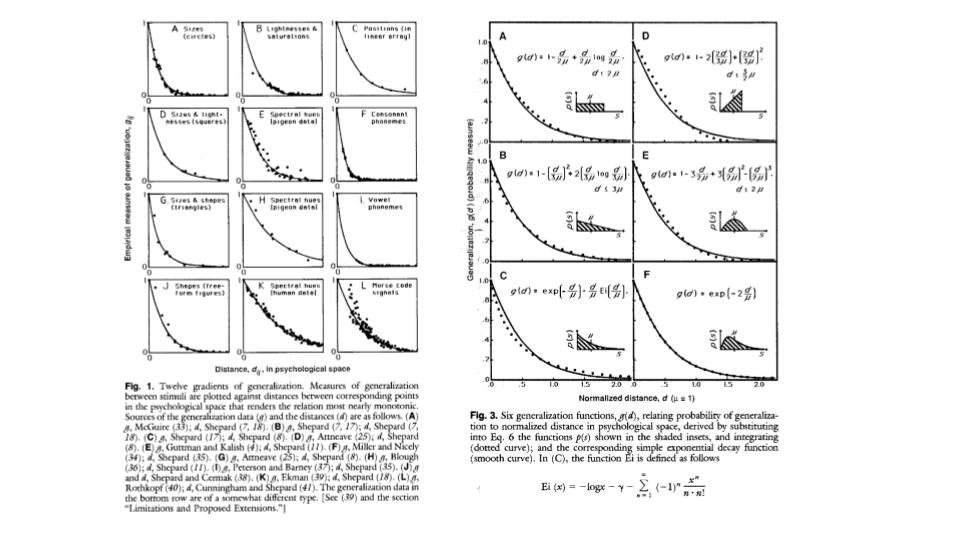
\includegraphics[width=5.8in]{shepard} \caption{Figures from Shepard's (1987) paper on stimulus generalisation. On the left (Figure 1 in the original) each of the 12 panels displays a generalization gradient, plotting the distance \(d_{ij}\) between the observed stimulus and the test stimulus in psychological space on the x-axis, and the empirical measure of generalization \(g_{ij}\) on the y-axis. The panels represent data from a variety of different species and stimulus domains. On the right (Figure 3 in the original), six theoretical generalization functions derived under different assumptions about \(p(s)\) (dotted lines), and the corresponding exponential decay. For additional detail see the original paper. \emph{{[}Note: if accepted, higher resolution versions will be provided in the final version and permission will be obtained to reproduce the originals{]}}}\label{fig:unnamed-chunk-1}
\end{figure}

Taken by itself Shepard's reanalysis would have been impressive. However, Shepard went on to provide a theoretical explanation for \emph{why} we should expect to find this invariance. The theory was surprisingly simple: the learner presumes there exists some unknown \emph{consequential} region of the stimulus space across which roughly the same properties hold (e.g., things that look like apples will probably taste the same as one another). Encountering a single stimulus that entails a particular consequence, the learner's task is to infer the location, shape and size of the consequential region itself. Naturally this is an underconstrained problem, as there are an infinite number of possible regions that might correspond to the true consequential region. Nevertheless, Shepard showed that under a quite range of assumptions that the learner might make about the nature of consequential regions, the shape of the \emph{generalization} function across the stimulus space ends up approximately exponential, shown on the right side of Figure 1.

Although brief, Shepard's paper has been highly influential in the cognitive science literature. It presented no new empirical data, and in substance it is mostly devoted to the derivation of a formal relation between one unobservable quantity (psychological distance) and another (generalisability). The universal law featured prominently in a special issue of \emph{Brain and Behavior Sciences} in 2001 and a first person retrospective (Shepard, 2004). In this special issue devoted to the prospects for theoretical development in psychology, I can think of no better case study to illustrate points I would like to make about the nature of theoretical work in psychology. My goal in this paper is to discuss the role that theory can play in the development of psychological science, using Shepard's law to illustrate.

\hypertarget{how-should-we-think-about-psychological-theories}{%
\section{How should we think about psychological theories?}\label{how-should-we-think-about-psychological-theories}}

\begin{quote}
\emph{I tentatively suggest that because these regularites reflect universal principles of natural kinds and of probabilistic geometry, natural selection may favor their increasingly close approximtion in sentient organisms wherever they evolve.} (Shepard, 1987, p.~1323)
\end{quote}

\noindent
Reading Shepard's original 1987 paper and the 2004 retrospective, some surprising characteristics of his theoretical work stand out. First, the theoretical development was largely post hoc. The paper does not collect new data, and indeed the main empirical results reported in the paper (left hand side of Figure 1) were based on a reanalysis of existing data. Second, the paper reports no hypothesis tests or indeed any statistical inference of any kind. There are no p-values, no Bayes factors, nor any confidence intervals or their Bayesian equivalents. Third, the paper does not outline any specific novel prediction about the result of future experiments. Though the paper makes a strong claim that the exponential law should hold broadly it does not prescribe how tests of this prediction should be constructed.

Viewed through the lens of the methodological reform culture (documented by Flis, 2019) all three of these properties might seem strange, and might even amount to a form of \enquote{questionable research practice}. To illustrate, consider the question of strong inference. In the current zeitgeist, strong claims cannot be justified without preregistered confirmatory tests (Wagenmakers, Wetzels, Borsboom, Maas, \& Kievit, 2012) but Shepard presents no tests at all while making sweeping claims. His theorising is entirely post hoc, and would at first blush appear to be a form of \enquote{HARKing} (hypothesizing after results are known; Kerr, 1998). Judged by the standards currently proposed for the assessment of psychological research, Shepard's paper might be expected to fare quite poorly. One might even be tempted to ask how Shepard managed to get the paper published at all.

Something seems awry in this description. Few researchers in the mathematical psychology community would consider Shepard (1987) to be ``bad science'' yet even a cursory inspection suggests it fails to meet some of the basic quality control criteria proposed as a remedy for the discipline's ills. The resolution to the discrepancy, I suggest, is that methodological criteria in psychology are typically developed to guide statistical inferences about empirical data, and -- as I have argued before (Navarro, 2019) -- are not well suited to the evaluation of scientific theories. Or to put it another way, one might argue that the success of Shepard's (1987) paper tells us a great deal about what a theory is not. Novel empirical data, no matter how fascinating or carefully collected, are not a theoretical contribution, and Shepard's theoretical work in his 1987 paper did not rely on a single new data set. Equally, a statistical test does not encapsulate what a theory does, and accordingly Shepard's theoretical contribution was neither reliant on nor presented as a statistical claim of any kind. Perhaps surprisingly, prediction and discovery need not lie at the core of a theoretical claim. The theoretical component to Shepard's paper was not the discovery of an exponential law, but rather the explanation proposed to account for it.

Empirical data, statistical inference and novel predictions are all vital to the scientific process -- of that there is little doubt -- but none of them are substitutes for or synonymous with theoretical development. If so, what might a theoretical explanation be? On my reading, what Shepard's paper did was \emph{systematise} an existing body of empirical findings. It separated those aspects to the data that are invariant across studies from those that are not. In doing so it provided a precisely stated mathematical formalism of those invariants that provide a conceptual framework to licence radical inferences beyond the scope of the original data. That is, while Shepard's theory asserts that the form of a generalisation curve should be exponential, this exponential law is not the theoretical primitive. Rather, the theoretical primitives are the assumptions Shepard made about consequential regions, psychological spaces, and the relationship these things have to stimulus generalisation.

It is precisely because his theory is built from such abstract primitives that Shepard justifies the generality of his claim. In short, the exponential law is an \emph{entailment} of the theory, not its substance. If the exponential law were merely observed in a few terrestrial species there would be little reason to suggest that the law should be expected to hold beyond our own planet. Such inference would be statistically unjustifiable, even as a \enquote{tentative suggestion}. Shepard makes this claim, not by relying on any statistical tool, but by noting that the exponential law emerges \emph{as} an entailment of more primitive rules that could be reasonably expected to hold in vastly different environments. It is this kind of \enquote{radical generalisation} that I argue is the key to good theorising.

\hypertarget{a-good-theory-can-escape-its-measurement-context}{%
\section{A good theory can escape its measurement context}\label{a-good-theory-can-escape-its-measurement-context}}

\noindent
In the remainder of this paper I want to use Shepard's law to motivate a discussion of what a good theory can achieve. Some desiderata for scientific theories seem easy to list. A scientific theory should be independent of its creator, for instance. It is difficult to make much use of a theory otherwise. In practice this typically means a theory is mathematical or computational in nature. Similarly, psychological theories should of course make some connection with empirical data, giving some account of the generative mechanism that gave rise to those data. Theories should be usable, in the sense of providing other scientists guidance for future research. Other criteria could also be named, including falsifiability, simplicity, compatibility with existing literature, generalizability, predictive ability and so on. However, while it is easy to list desiderata and even easier to argue over which elements to such lists are the most important, such ``discussions in the abstract'' rarely provide much guidance to the would-be theoretician. From the perspective of the working scientist, it is perhaps more useful to give concrete examples, and to that end I return to an examination of Shepard's (1987) paper.

Consider first the problem of measurement. If one is to build a strong theory, it must be tethered in some way to observational or experimental data, and to do so one must have an appropriate measurement tool. For example, one of the key insights in Shepard's (1987) paper is the recognition that stimulus generalization functions that appear extremely irregular at first glance are in fact highly regular when stimuli are represented in an appropriate fashion, as depicted in Figure 2. Generalization to tones is irregular when tones are described in terms of their ordering around the chroma circle, but very smooth when described around the circle of fifths. Similarly, stimulus generalization to colours is irregular with respect the physical wavelenghts of light but is smooth with respect to perceptual colours space (e.g., Ekman, 1954). In retrospect this seems obvious, but at the time Shepard developed the theory, he was faced with a substantive problem of how to extract the \emph{appropriate} stimulus representation to apply a theory to. Nonmetric multidimensional scaling (MDS; Kruskal, 1964) as a measurement instrument tool served this purpose for Shepard in 1987, and the smooth empirical curves on the left of Figure 1 all use MDS-estimated psychological spaces to supply the relevant measure of distance on the x-axis.



\begin{figure}[t]
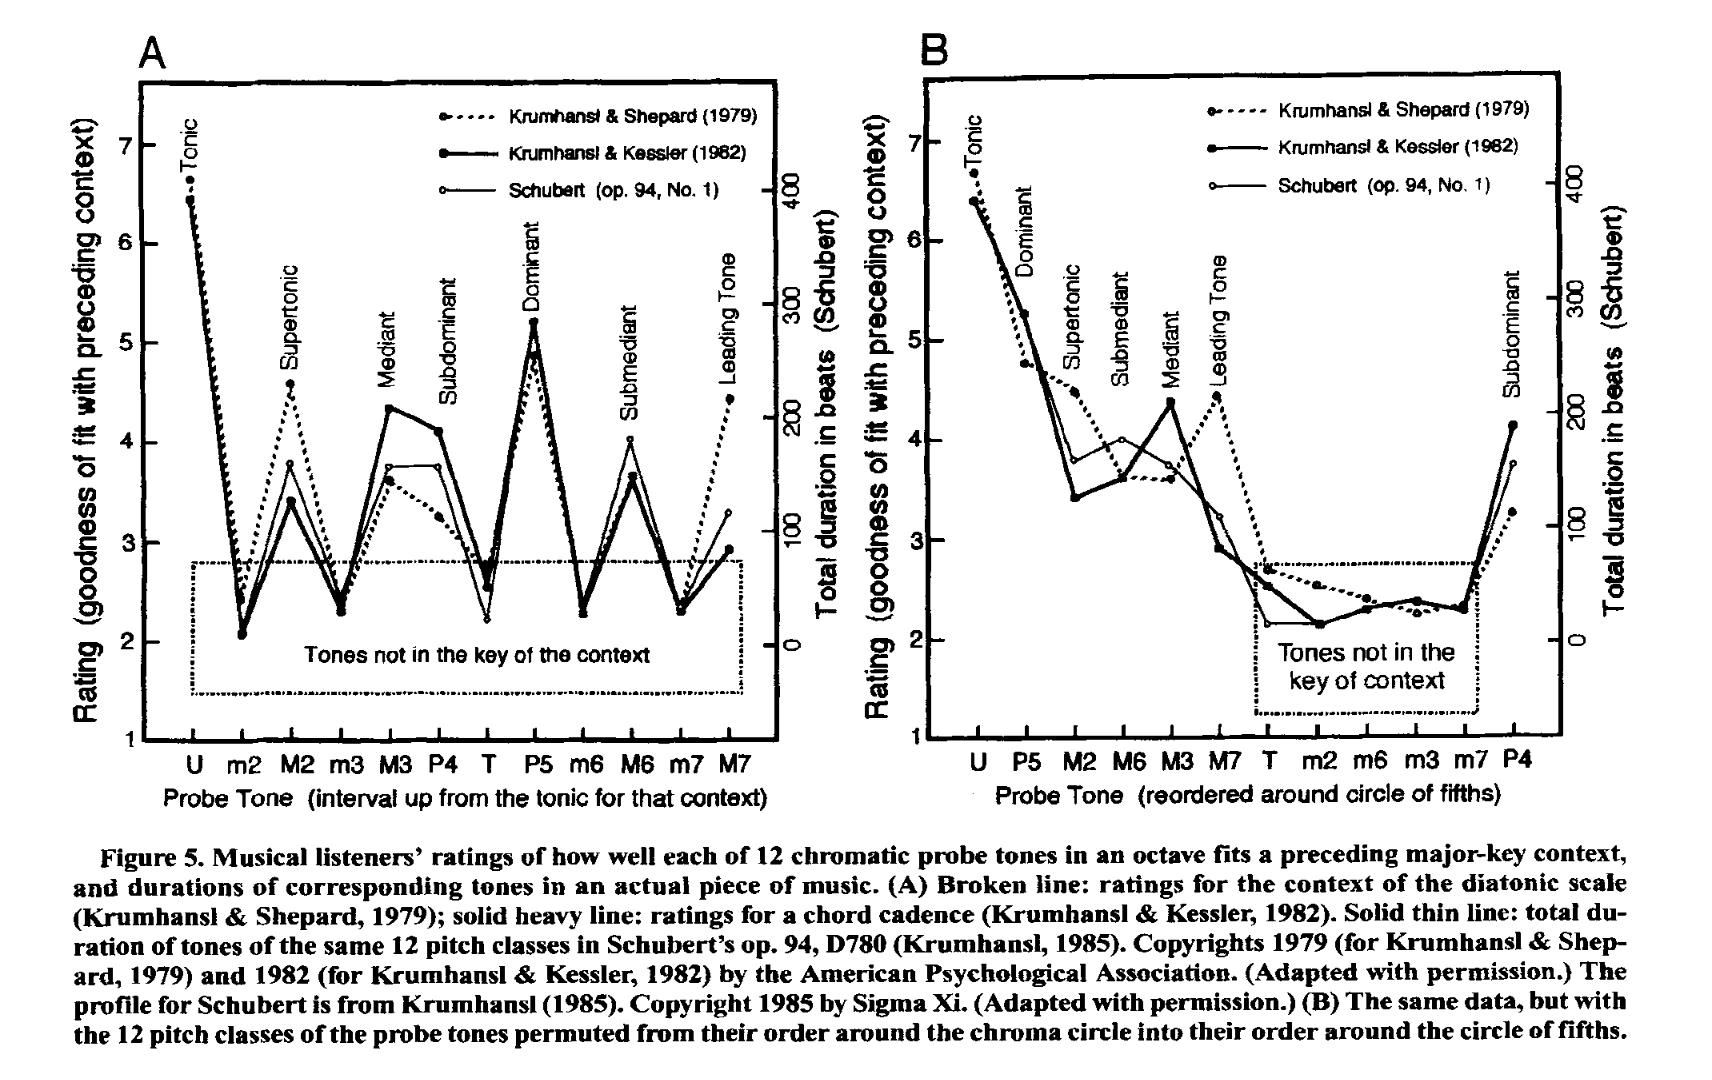
\includegraphics[width=5.51in]{shepard2} \caption{Illustrations taken from Shepard's (2004) retrospective account of the universal law, plotting stimulus generalization data from three previous experiments in two different formats. On the left, data are shown in a raw format, and on the right data are recast in terms of constructs relevant to the theory. See original for more detail. \emph{{[}Note: a higher resolution version will be provided in the final version and permission will be obtained to reproduce the originals{]}}}\label{fig:unnamed-chunk-2}
\end{figure}

As this discussion illustrates, without MDS as a measurement tool Shepard would have found it almost impossible to formulate the empirical regularity with any confidence. However, it is equally clear that MDS is merely a tool used to help define the phenomenon to be explained. It does not define the theory itself, and in the relevant literature it quickly became apparent that Shepard's law applies even in situations where MDS does not: shortly after the publication of Shepard's original paper, Russell (1988) demonstrated that the same law holds for stimuli defined in terms of discrete features as well as to the continuous spaces for which Shepard's work was defined, a connection that was later extended by Tenenbaum and Griffiths (2001). While the theoretical framework could not have come into existence without the scaffolding provided by the MDS measurement model, it quickly outgrew any need for this support. Illustrating this, the generalization gradient shown in Figure 3 is neither exponential in superficial form, nor is the underlying stimulus representation a metric space extracted by MDS, yet as Tenenbaum and Griffiths (2001) note, it too can be seen as an entailment of Shepard's theoretical framework.



\begin{figure}[t]
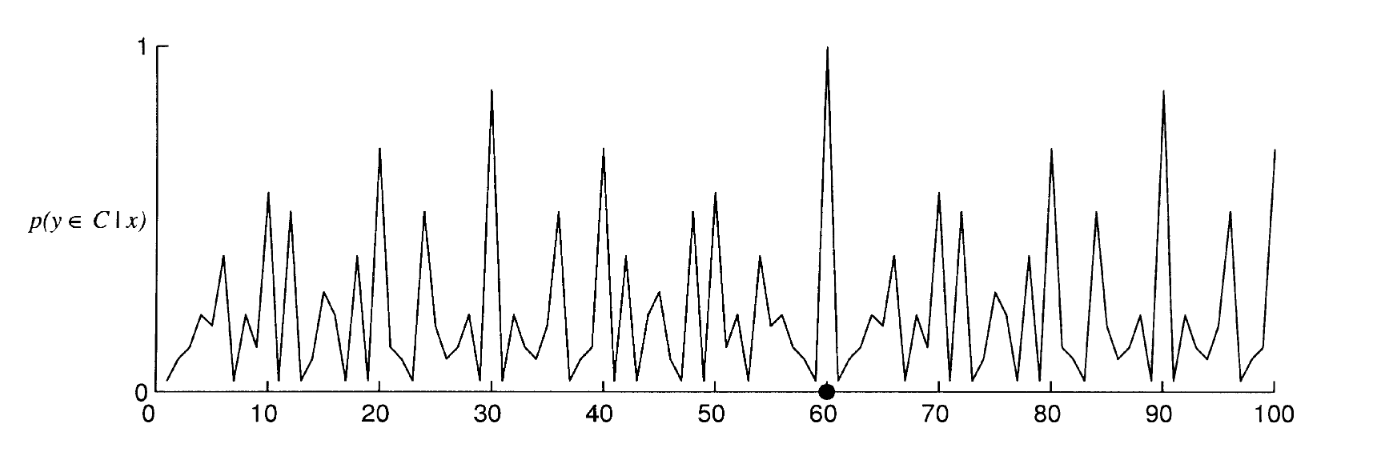
\includegraphics[width=4.58in]{tenenbaum_figure5} \caption{A Bayesian generalization gradient for stimuli (numbers) that are more naturally represented in terms of discrete consequential sets, reproduced from Tenenbaum and Griffiths (2001). In this example, the learner knows that a property holds for the number ``60'', and must judge the probability that this novel property holds for other numbers. The hypothesis space \(\mathcal{H}\) consists of sets of consecutive numbers (to capture the notion that people are sensitive to magnitude), but also includes a variety of mathematical properties (even numbers, odd numbers, multiples of three, etc). See original for more detail. \emph{{[}Note: a higher resolution version will be provided in the final version and permission will be obtained to reproduce the originals{]}}}\label{fig:unnamed-chunk-3}
\end{figure}

\hypertarget{a-good-theory-can-escape-its-formal-description}{%
\section{A good theory can escape its formal description}\label{a-good-theory-can-escape-its-formal-description}}

\noindent
The second point to consider is the role of formalism. The mathematical form that Shepard used to implement his ideas is not unique, and the theory can be rewritten in different notation. Previously, Cooper and Guest (2014) have argued that theoretical work need not be constrained to a particular \enquote{implementation} (or formalism), but is better captured by a more abstract notion of a \enquote{specification}. As a concrete example, it is worth considering the manner in which Shepard's law was later reformulated as a Bayesian model,\footnote{Because Bayesian inference is often considered to be a normative standard for learning, it should be noted that some care is required in assigning normative status to Bayesian models of cognition; see Tauber, Navarro, Perfors, and Steyvers (2017).} and the effect this rewriting had on how the model could be applied.

In his original notation Shepard proposed that the generalization strength for a stimulus located at coordinate \(\mathbf{x} = (x_1, \ldots, x_K)\) in a \(K\)-dimensional space,\footnote{The space is usually endowed with one of the Minkowski distance metrics, most typically the Euclidean distance measure or the city block distance. One of the major contributions Shepard made was to provide a theoretical explanation for why the distance metric varies across stimulus domains, but is a little beyond the scope of the current paper.} when the learner has previously encountered a consequential stimulus located at the origin be expressed as follows:

\begin{equation}
g(\mathbf{x}) = \int_0^\infty p(s) \frac{m(s, \mathbf{x})}{m(s)} ds
\end{equation}

\noindent
where the ratio \(m(s, \mathbf{x})/m(s)\) is a measure describing the probability that a consequential region of size \(s\) contains \(\mathbf{x}\) given that it also contains the consequential stimulus at the origin, and \(p(s)\) is a probability measure that assigns value to regions of size \(s\). Much of Shepard's paper is devoted to solving this integral for various choices of \(p(s)\) and showing that the resulting generalization function \(g(\mathbf{x})\) is approximately exponential in form, and is precisely exponential when \(p(s)\) is the Erlang distribution.

In and of itself Equation 1 does not describe a Bayesian model. The connection to Bayesian inference was made explicit by Tenenbaum and Griffiths (2001) who recast Shepard's formalism using different notation and expressing the underlying ideas rather differently. Where Shepard referred to the notion of a \enquote{consequential region} located within a psychological space with all the geometric connotations that entails, Tenenbaum and Griffiths took a more general view and framed their analysis in terms of \enquote{consequential sets}. Any specific candidate for the true consequential set was labelled a \enquote{hypothesis} \(h\), presumed to belong to a broader \enquote{hypothesis space} \(\mathcal{H}\). In their notation, the measure on regions sizes \(p(s)\) was replaced by a Bayesian prior \(p(h)\) defined over the hypothesis space, and Shepard's ratio \(m(s, \mathbf{x})/m(s)\) recast in probabilistic terms also. In their notation, the probability of generalising to a novel stimulus \(y\) given that a consequential stimulus \(x\) has already been observed is formulated as the following Bayesian marginal probability:

\begin{equation}
p(y \in C | x) = \sum_{h : y \in C} p(h|x)
\end{equation}
\noindent
where \(p(h|x)\) is the posterior probability a Bayesian learner assigns to hypothesis \(h\) in light of observing the consequential stimulus \(x\),
\begin{equation}
p(h|x) = \frac{p(x|h)p(h)}{\sum_{h^\prime \in \mathcal{H}} p(x | h^\prime) p(h^\prime)}
\end{equation}
where \(p(x|h)\) is the likelihood that the learner would encounter the data \(x\) if hypothesis \(h\) were true, and the summation in the denominator is taken over all hypotheses in the learner's hypothesis space.

The Bayesian reformulation of Shepard's theory presented by Tenenbaum and Griffiths was more than a superficial change: it allowed them to show how Shepard's theory could itself be generalized in three distinct ways. First, as mentioned earlier, they showed (much like Russell 1988) that Shepard's theory could encompass stimuli that were not representable as points in a metric space: in their notation, this is as accomplished by substituting a new hypothesis space \(\mathcal{H}\). Second, this formulation allowed the theory to naturally accommodate inductive generalization problems in which the learner has encountered more than one consequential stimulus. If a set of \(n\) stimuli \(\mathbf{x} = (x_1, \ldots, x_n)\) are generated in a (conditionally) independent fashion, the likelihood \(p(\mathbf{x}|h)\) factorises and thus
\begin{equation}
p(\mathbf{x}|h) = \prod_{i=1}^n p(x_i |h).
\end{equation}
Finally, this formalism called attention to a potentially limiting assumption in Shepard's original paper. Shepard (1986, p.~1321) argued that ``in the absence of any information to the contrary, an individual might best assume that nature selects the consequential region and the first stimulus independently''. According to this account, which Tenenbaum and Griffiths termed \emph{weak sampling}, this independence gives a uniform likelihood function:
\begin{equation}
p(x|h) \propto 1
\end{equation}
They contrasted this with a \emph{strong sampling} account in which stimuli are presumed to be sampled uniformly from the consequential set. If \(|h|\) denotes the size of the consequential set\footnote{For finite sets this \(|h|\) is simply the number of entities in the set; for infinite sets, a more careful approach to measuring the size of sets is required} then a strong sampling process produces the likelihood
\begin{equation}
p(x|h) = 1/|h|
\end{equation}
if \(x\) is an element of the consequential set, and 0 otherwise.

While a complete description of the relationship between Shepard's formalism and Tenenbaum and Griffiths' is beyond the scope of this paper, some things seem clear enough. In one sense the two formalisms capture the \enquote{same} underlying theoretical idea, but that does not make them equivalent. As I outlined above, the Bayesian reformulation encourged researchers to apply the model in different ways. By \enquote{escaping} the original notation Shepard used to describe it, the theory could be extended to quite different problems, as I describe in the next section.

\hypertarget{a-good-theory-can-escape-its-empirical-domain}{%
\section{A good theory can escape its empirical domain}\label{a-good-theory-can-escape-its-empirical-domain}}

\noindent
The third point I wish to consider is the way in which theories can extend their domain of applicability. Looking at their paper in retrospect, one of the most important contributions made by the Bayesian formulation adopted by Tenenbaum and Griffiths (2001) is that it allowed the underlying theory to be applied in a much broader range of scenarios. Shepard's (1987) original construction, though purportedly to be a very general law itself, was formulated with respect to a narrow class of psychological problems: inductive generalization from a single observation. Moreover, because the origins of his work lay in the study of human perception and the animal learning literature, it was not immediately clear -- at least it was not clear to me -- how the theory should be extended to higher order cognition. By framing the problem in a more general way, Tenenbaum and Griffiths' construction enabled a large proportion of my later research. Examples of research questions that I would have been unable to properly formulate without this theory:

\begin{itemize}
\tightlist
\item
  What kind of individual differences exist in the sampling assumptions people adopt in simple generalization problems? (Navarro, Dry, \& Lee, 2012)
\item
  Do categorization problems and inductive generalization problems lead people to adopt different sampling assumptions? (Hendrickson, Perfors, Navarro, \& Ransom, 2019)
\item
  Do people's beliefs about the origins of data and shape how we interpret the evidentiary value of the quantity (Ransom, Perfors, \& Navarro, 2016) and diversity of evidence (Hayes et al., 2019b)?
\item
  Can we use the Bayesian theory to unify and extend previously puzzling results (Lawson \& Kalish, 2009) on how sampling affects reasoning? (Hayes et al., 2019a)
\item
  Can we build a Bayesian model of how people ``take a hint'' from ostensibly uninformative data? (Voorspoels, Navarro, Perfors, Ransom, \& Storms, 2015)
\item
  Completing a ``virtuous cycle'' of sorts, recent work has taken our results from the reasoning context (Voorspoels et al., 2015) and applied it to make novel predictions in the associative learning (Lee, Lovibond, Hayes, \& Navarro, 2019)
\end{itemize}

This is of course a highly selected portion of the relevant literature, focusing as it does on work in which I was personally involved. The purpose of choosing these examples is that -- as the person developing the theoretical extensions in each case -- I am in a position to comment on exactly \emph{how} the theoretical formalism from Tenenbaum and Griffiths (2001) paper enabled this research when the original formalism from Shepard (1987) would have made it difficult. Because Shepard's formalism adhered closely to the specific problem he sought to explain (generalization from a single observed stimulus represented in a metric space) it was not clear to me prior to 2001 that the learner is necessarily reliant on an assumption (explicit or implicit) about how the stimulus was called to the learner's attention. Under the Bayesian reformulation of the theory, this assumption was rendered visible via the likelihood \(P(x|h)\). When written in this form, it was painfully clear to me that the inductive inferences any learner makes about a novel item \(y\) is necessarily dependent on more than the observed data \(x\) -- it also depends on the assumptions embodied in the likelihood \(P(\cdot|h)\) as to how those data were collected. This link, present but obscured in Shepard's (1987) paper, was the central motivation behind this entire body of work and would not have been possible without the more abstract formalism introduced by Tenenbaum and Griffiths (2001).

\hypertarget{conclusion}{%
\section{Conclusion}\label{conclusion}}

\begin{quote}
\emph{Those outside the field, on hearing the term mathematical psychology, often react with the raised eyebrows reserved for oxymora} (Shepard, 2004, p. 1)
\end{quote}

\noindent
Mathematical psychology is something of an oddity in the discipline. It does not eschew empirical research, but neither does it view the goal of science to be the accrual of empirical effects. Quite unlike most areas of psychology with which I am familiar, mathematical psychologists place a high value on theoretical development, particularly when such theories can be stated in a formal manner. My goal in this paper was to highlight the manner in which cumulative theoretical work has developed in this discipline, using Shepard's law as an example. From its origins in associative learning and stimulus generalization, to its reformulation as a Bayesian model and its extension to a variety of novel contexts, a single theoretical claim can be shown to connect to a variety of empirical findings in superficially distinct domains. The breadth of situations to which the law can be unambiguously applied is greatly to be desired in a theoretical explanation.

Although I have focused on Shepard's law and its extensions in this paper, the underlying pattern is -- I would suggest -- quite general. I could have chosen the Rescorla-Wagner model of associative learning as the basis for this discussion (Rescorla \& Wagner, 1972), or the Generalized Context Model of human categoriztion (Nosofsky, 1986). I could have chosen to focus on models such as ALCOVE that sought to unify associative learning and categorization (Kruschke, 1992), or models such as the hierarchical Dirichlet process that seek to unify a wide variety of category learning models within a common theoretical language (Griffiths, Canini, Sanborn, \& Navarro, 2007). I could have revisited Ebbinghaus' 1885 work on formal theory in experimental psychology (reprinted as Ebbinghaus, 2013). I could have examined sequential sampling models of choice reaction time (Luce, 1986) and the rich theoretical tradition that mathematical psychologists have developed in that domain also.

These theoretical advances have something in common. In each of these areas psychological researchers have built up a considerable body of theoretical knowledge that is instantiated in formal models of psychological processes. In every case the underlying theoretical models are more than mere summaries of empirical results, and more substantive than a mere statistical model. In all cases the formalism can be used to generate novel predictions in experimental paradigms that differ markedly from the experimental contexts used to develop the model (and, remarkably, some of those predictions have even turned out to be correct). By a judicious combination of abstraction and formalism, mathematical psychologists have been able to develop a toolkit that allows anyone to derive theoretical predictions in completely novel paradigms. If it is indeed the case that psychology suffers from a kind of ``theoretical amnesia'' (Boorsbaum, 2013), perhaps the machinery of mathematical psychology can aid its memory. Perhaps fittingly, the words of Shepard (1987, p.~1323) seem an appropriate way to conclude

\begin{quote}
\emph{Undoubtably, psychological science has lagged by behind physical science by at least 300 years. Undoubtedly, too, prediction of behavior can never attain the precision for animate that it has for celestial bodies. Yet, psychology may not be inherently limited merely to the descriptive characterization of the behaviors of particular terrestrial species. Possibly, behind the diverse behaviors of humans and animals, as behind the various motions of planets and stars, we may discern the operation of universal laws}
\end{quote}

\hypertarget{references}{%
\section{References}\label{references}}

\hypertarget{refs}{}
\leavevmode\hypertarget{ref-boorsbaum2013theoretical}{}%
Boorsbaum, D. (2013). Theoretical amnesia. \emph{Center for Open Science}. Retrieved from \url{http://osc.centerforopenscience.org/2013/11/20/theoretical-amnesia/}

\leavevmode\hypertarget{ref-cooper2014implementations}{}%
Cooper, R. P., \& Guest, O. (2014). Implementations are not specifications: Specification, replication and experimentation in computational cognitive modeling. \emph{Cognitive Systems Research}, \emph{27}, 42--49.

\leavevmode\hypertarget{ref-ebbinghaus2013memory}{}%
Ebbinghaus, H. (2013). Memory: A contribution to experimental psychology. \emph{Annals of Neurosciences}, \emph{20}(4), 155.

\leavevmode\hypertarget{ref-ekman1954dimensions}{}%
Ekman, G. (1954). Dimensions of color vision. \emph{The Journal of Psychology}, \emph{38}(2), 467--474.

\leavevmode\hypertarget{ref-Flis2019}{}%
Flis, I. (2019). Psychologists psychologizing scientific psychology: An epistemological reading of the replication crisis. \emph{Theory \& Psychology}, \emph{29}(2), 158--181.

\leavevmode\hypertarget{ref-griffiths2007unifying}{}%
Griffiths, T., Canini, K., Sanborn, A., \& Navarro, D. (2007). Unifying rational models of categorization via the hierarchical dirichlet process.

\leavevmode\hypertarget{ref-hayes2019selective}{}%
Hayes, B. K., Banner, S., Forrester, S., \& Navarro, D. J. (2019a). Selective sampling and inductive inference: Drawing inferences based on observed and missing evidence. \emph{Cognitive Psychology}, \emph{113}, 101221.

\leavevmode\hypertarget{ref-hayes2019diversity}{}%
Hayes, B. K., Navarro, D. J., Stephens, R. G., Ransom, K., \& Dilevski, N. (2019b). The diversity effect in inductive reasoning depends on sampling assumptions. \emph{Psychonomic Bulletin \& Review}, \emph{26}(3), 1043--1050.

\leavevmode\hypertarget{ref-hendrickson2019sample}{}%
Hendrickson, A. T., Perfors, A., Navarro, D. J., \& Ransom, K. (2019). Sample size, number of categories and sampling assumptions: Exploring some differences between categorization and generalization. \emph{Cognitive Psychology}, \emph{111}, 80--102.

\leavevmode\hypertarget{ref-kerr1998harking}{}%
Kerr, N. L. (1998). HARKing: Hypothesizing after the results are known. \emph{Personality and Social Psychology Review}, \emph{2}(3), 196--217.

\leavevmode\hypertarget{ref-kruschke1992alcove}{}%
Kruschke, J. K. (1992). ALCOVE: An exemplar-based connectionist model of category learning. \emph{Psychological Review}, \emph{99}(1), 22.

\leavevmode\hypertarget{ref-kruskal1964nonmetric}{}%
Kruskal, J. B. (1964). Nonmetric multidimensional scaling: A numerical method. \emph{Psychometrika}, \emph{29}(2), 115--129.

\leavevmode\hypertarget{ref-lawson2009sample}{}%
Lawson, C. A., \& Kalish, C. W. (2009). Sample selection and inductive generalization. \emph{Memory \& Cognition}, \emph{37}(5), 596--607.

\leavevmode\hypertarget{ref-lee2019negative}{}%
Lee, J. C., Lovibond, P. F., Hayes, B. K., \& Navarro, D. J. (2019). Negative evidence and inductive reasoning in generalization of associative learning. \emph{Journal of Experimental Psychology: General}, \emph{148}(2), 289.

\leavevmode\hypertarget{ref-luce1986response}{}%
Luce, R. D. (1986). \emph{Response times: Their role in inferring elementary mental organization}. Oxford University Press on Demand.

\leavevmode\hypertarget{ref-navarro2019between}{}%
Navarro, D. J. (2019). Between the devil and the deep blue sea: Tensions between scientific judgement and statistical model selection. \emph{Computational Brain \& Behavior}, \emph{2}(1), 28--34.

\leavevmode\hypertarget{ref-navarro2012sampling}{}%
Navarro, D. J., Dry, M. J., \& Lee, M. D. (2012). Sampling assumptions in inductive generalization. \emph{Cognitive Science}, \emph{36}(2), 187--223.

\leavevmode\hypertarget{ref-nosofsky1986attention}{}%
Nosofsky, R. M. (1986). Attention, similarity, and the identification--categorization relationship. \emph{Journal of Experimental Psychology: General}, \emph{115}(1), 39.

\leavevmode\hypertarget{ref-ransom2016leaping}{}%
Ransom, K. J., Perfors, A., \& Navarro, D. J. (2016). Leaping to conclusions: Why premise relevance affects argument strength. \emph{Cognitive Science}, \emph{40}(7), 1775--1796.

\leavevmode\hypertarget{ref-rescorla1972theory}{}%
Rescorla, R. A., \& Wagner, A. R. (1972). A theory of pavlovian conditioning: Variations in the effectiveness of reinforcement and nonreinforcement. \emph{Classical Conditioning II: Current Research and Theory}, \emph{2}, 64--99.

\leavevmode\hypertarget{ref-russell1988analogy}{}%
Russell, S. (1988). Analogy by similarity. In \emph{Analogical reasoning} (pp. 251--269). Springer.

\leavevmode\hypertarget{ref-shepard1987toward}{}%
Shepard, R. N. (1987). Toward a universal law of generalization for psychological science. \emph{Science}, \emph{237}(4820), 1317--1323.

\leavevmode\hypertarget{ref-shepard2004cognitive}{}%
Shepard, R. N. (2004). How a cognitive psychologist came to seek universal laws. \emph{Psychonomic Bulletin \& Review}, \emph{11}(1), 1--23.

\leavevmode\hypertarget{ref-tauber2017bayesian}{}%
Tauber, S., Navarro, D. J., Perfors, A., \& Steyvers, M. (2017). Bayesian models of cognition revisited: Setting optimality aside and letting data drive psychological theory. \emph{Psychological Review}, \emph{124}(4), 410.

\leavevmode\hypertarget{ref-tenenbaum2001generalization}{}%
Tenenbaum, J. B., \& Griffiths, T. L. (2001). Generalization, similarity, and bayesian inference. \emph{Behavioral and Brain Sciences}, \emph{24}(4), 629--640.

\leavevmode\hypertarget{ref-voorspoels2015people}{}%
Voorspoels, W., Navarro, D. J., Perfors, A., Ransom, K., \& Storms, G. (2015). How do people learn from negative evidence? Non-monotonic generalizations and sampling assumptions in inductive reasoning. \emph{Cognitive Psychology}, \emph{81}, 1--25.

\leavevmode\hypertarget{ref-Wagenmakers2012}{}%
Wagenmakers, E.-J., Wetzels, R., Borsboom, D., Maas, H. L. van der, \& Kievit, R. A. (2012). An agenda for purely confirmatory research. \emph{Perspectives on Psychological Science}, \emph{7}, 632--638.

\end{document}
